\documentclass[11pt]{article}
\usepackage{geometry}
\geometry{
 a4paper,
 total={210mm,297mm},
 left=20mm,
 right=20mm,
 top=20mm,
 bottom=20mm,
 }
 
\usepackage[english]{babel}
\usepackage[utf8x]{inputenc}
\usepackage{amsmath}
\usepackage{graphicx}
\usepackage[colorinlistoftodos]{todonotes}
\usepackage{multicol}
\usepackage{ragged2e}
\usepackage{tocloft}
\usepackage{gensymb}
\usepackage{siunitx}
\usepackage[hypcap]{caption}
\usepackage{capt-of}
\usepackage{setspace}
\usepackage[parfill]{parskip}
\usepackage{amssymb}
\usepackage{textcomp}
\usepackage{float}
\floatstyle{plain}
\usepackage{color}
\usepackage{epstopdf}
\usepackage{natbib}
\usepackage{hyperref}
\hypersetup{
    colorlinks=true,
    linkcolor=blue,
    filecolor=magenta,      
    urlcolor=cyan,
    citecolor=blue
}
\urlstyle{same}

%abstract
\renewenvironment{abstract}
 {\hspace{.8cm}
  {\bfseries\Large\abstractname}
  \list{}{
    \setlength{\leftmargin}{.95cm}%
    \setlength{\rightmargin}{\leftmargin}%
  }%
  \item\relax}
 {\endlist}

%random things needed
%\renewcommand{\cftsecleader}{\cftdotfill{\cftdotsep}} %let the content table have dots to number
\linespread{1.5}  %making one and a half spacing-sh one and half is actually 1.3
\frenchspacing


\begin{document}
\begin{titlepage}
	\centering
	\topskip0pt
	\vspace*{\fill}
	{\huge\bfseries Developing a purification strategy \\ for Cas9\par}
	\vspace{2cm}
	{\Large Jia Le, Lim {    }  CID: 00865029}
	\\ 	\vspace{0.5cm}
	{Department of Biology, Imperial College London, \\South Kensington Campus, London, U.K.} \\ \vspace{0.5cm}
	{Interned at: Protein Expression and Purification Core Facility, \\European Molecular Biology Laboratory,\\ Heidelberg, Germany} \\
	\vspace*{\fill}
	{\large Supervised by\par
	Dr.~Kim \textsc{Remans} \& Ms Ines \textsc{Racke} }
	\vfill
% Bottom of the page
	{\large Submitted: \today\par}
\end{titlepage}

\vspace*{\fill}
\tableofcontents 
\vspace*{\fill} 
\thispagestyle{empty}

\doublespacing

\newpage
\pagenumbering{gobble}
\vspace*{\fill}
\begin{abstract}  
\doublespacing
The Clustered Regularly Interspaced Short Palindromic Repeats (CRISPR) and CRISPR-associated (Cas) protein system is naturally found in prokaryotes as an adaptive immune response against pathogens. Cas9 proteins interact with double-stranded RNAs to target and cleave exogenous DNA. This system has also been adapted to create genetic modifications in transgenic cells in order to investigate the roles and functions of genes. In this paper, a purification protocol for types of Cas9 proteins has been modified from \cite{Jinek2012a} and tested to provide a cheap, reliable and flexible source of Cas9 proteins required for molecular biology research. 

\end{abstract}
\vfill


\newpage
\pagenumbering{arabic}
\section{Introduction} 
\subsection{Clustered Regularly Interspaced Short Palindromic Repeats (CRISPR)}
Clustered Regularly Interspaced Short Palindromic Repeats (CRISPR) is an adaptive immune response used by prokaryotes~\citep{Sorek2013}.  Each CRISPR locus comprises of short repeat sequences interrupted by unique spacer sequences derived from viral elements. CRISPR-associated (Cas) proteins bind to the CRISPR RNAs (crRNAs) transcribed from CRISPR loci, creating ribonucleoproteins (RNP) that target and cleave viral sequences complementary to crRNA, hence preventing viral infections~\citep{Jiang2015, Sternberg2015}. 

There are three main types of CRISPR-Cas systems. Type I and III CRISPR-Cas systems consist of large complexes of proteins. These systems are therefore not feasible for experimental use as multiple genes or proteins have to be simultaneously introduced into the cell for the CRISPR-Cas system to be functional. The Type II system, on the other hand, consists of only one protein, Cas9. This system was therefore chosen for genome engineering~\citep{Doudna2014, Jinek2012a}.

\subsection{Genome engineering}
The main aim of genome engineering is the introduction of site-specific modifications to targeted genes. In recent years, zinc finger nucleases (ZFNs) and transcription activator-like effector nucleases (TALENs) have been popular in this field. These proteins, when coupled to nuclease domains of restriction enzymes, were able to directly bind DNA and create a double-stranded break (DSB) at specific sites. However, new DNA-binding proteins have to be designed to target novel DNA sequences. The design, expression and validation of such proteins are difficult and problematic as ZFNs and TALENS directly bind to targeted sequences~\citep{Doudna2014}.

Another conventional method involves the use of RNA interference (RNAi). Small RNAs are designed to be complementary to the targeted RNA. When introduced into cells, RNAi binds to mRNAs of interest. This results in double-stranded RNAs that will be degraded by eukaryotic cells. This method reduces the expression of proteins of interest but has been shown to have unpredictable off-target effects and is unable to completely inhibit gene expression. Moreover, RNAi mainly targets mRNA and its inhibition of gene expression is only temporary~\citep{Gilles2014a}.

\subsection{Type II CRISPR-Cas system}
The DNA endonuclease Cas9 contains two nuclease domains homologous to HNH and RuvC endonucleases. In this system, the crRNA forms a double-stranded structure with the trans-activating crRNA (tracrRNA). This double-stranded RNA binds to Cas9 proteins and directs it to the targeted DNA base-paired with crRNA. Thereafter, Cas9 protein creates a DSB three base pairs upstream of the Protospacer adjacent motif (PAM)~(\autoref{fig:gRNA.png}). PAM is used by prokaryotes to differentiate between exogenous and intracellular DNA and must be found in targeted DNA sequences for DSB to occur~\citep{Jinek2012a}. In \textit{Streptococcus pyogenes}, the PAM sequence is NGG and this limits the range of DNA targets by the \textit{Streptococcus pyogenes} Cas9 (SpyCas9) protein in mammalian cells. Cas9 proteins from different bacteria have differing PAM sequences and these can help in increasing the range of nucleotide sequences the Cas9 can target. ~\citep{Hou2013a}

Nonetheless, Cas9 proteins can bind to a single chimeric RNA or guide RNA (gRNA) designed to form a double-stranded structure similar to that of crRNA:tracrRNA duplex~(\autoref{fig:gRNA.png}). By changing the 20bp protospacer of the gRNA, researchers can easily manipulate the Cas9 to cleave their genes of interest. This can be performed easily by subcloning the nucleotide sequence into the gRNA backbone plasmidMoreover, with the introduction of multiple gRNAs, multiple genes can be modified simultaneously~\citep{Jinek2012a}. Hence, Cas9 is becoming increasingly popular as little time is required for the design of the gRNA.

\begin{figure}[H]
  \centering
    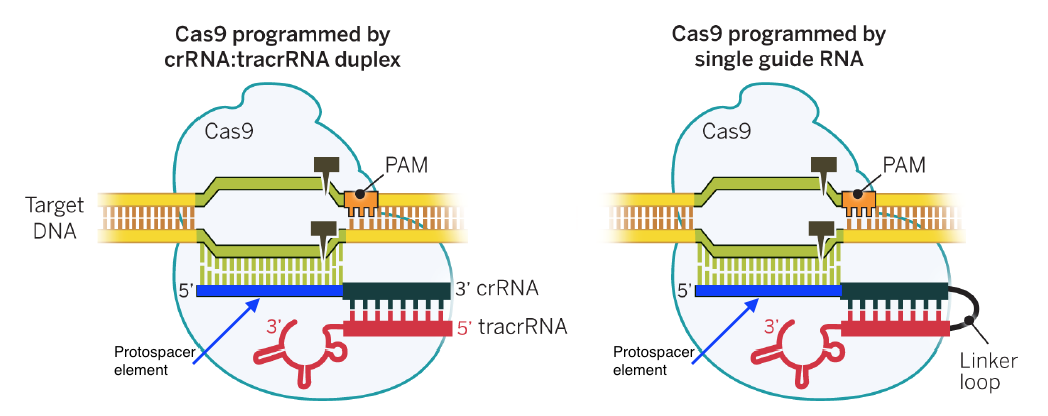
\includegraphics[width=\textwidth, height = 60mm]{gRNA.png}
  \captionof{figure}{\footnotesize Structure of Cas9. HNH and RuvC-like domains each cut a single strand of DNA at a site three base pairs upstream of the Protospacer adjacent motif (PAM), creating a double-stranded break. Figure obtained from~\cite{Doudna2014}.}
    \label{fig:gRNA.png}
\end{figure}

Cas9 proteins are also considerably smaller than TALENs and ZFNs. This allows the use of many potential viral and non-viral delivery vehicles, such as self-inactivating lentivirus and lipid nanoparticles, to deliver Cas9 and its gRNA cDNA into cells. Electroporation or lipid-based transfection can also be used to successfully introduce the RNP complex into cells~\citep{Gori2015}.

DSBs created by Cas9 proteins induce homology-directed repair or inaccurate repair by non-homologous end joining (NHEJ), mechanisms commonly found in cells. Such mechanisms introduce indels at the site of DSB, hence disrupting gene function. Thus, the creation of DSBs has been the rate-limiting step in genome modifications and this limitation has been mitigated by the use of CRISPR-Cas9 system~\citep{Chen2015a, Ramalingam2013}. 

\subsection{Cas9 Variants}
Besides the SpyCas9 protein, many mutant forms of SpyCas9 were subsequently created and applied to varying types of research. 

Cas9 D10A nickase and Cas9 H840 nickase were created with a non-functional HNH or RuvC endonuclease respectively. Cas9 nickases create a DSB when they both cause nearby single-stranded breaks, hence reducing off-target DSB caused by single Cas9 nucleases~\citep{Ran2013}. 

Another method of reducing unwanted DSB is to attach Fok1 endonucleases to dead Cas9(dCas9) proteins. When dCas9 proteins bind to targeted DNA in the vicinity of another dCas9, Fok1 dimerises and creates a DSB. dCas9 proteins have non-functional endonuclease activity but similarly bind to DNA complementary to gRNA~\citep{Guilinger2014c}. Due to its DNA-binding activity, transcriptional repressors and activators have also been coupled to dCas9 to conduct genome-scale screens for essential genes, tumor suppressor genes, drug resistance genes and others~\citep{Gilbert2014, Shalem2015}. 

With the numerous Cas9 variants, Cas9 proteins are hence becoming increasingly relevant to many different fields of molecular biology.

\subsection{Project aim}
Cas9 proteins are currently available commercially (Thermo Fisher Scientific Inc., New England BioLabs). However, the commonly available Cas9 proteins are the wild type SpyCas9 nucleases and Cas9 nickases. With increasingly more uses of Cas9 proteins being discovered, many different variants of Cas9 needs to be produced, such as recombinant dCas9, for varying research aims. Currently, most research involving the Cas9 infects their cells with 

As such, the Protein Expression and Purification Core Facility at the European Molecular Biology Laboratory(EMBL), Heidelberg hope to be able to provide a cheaper, faster and more flexible alternative for the other researchers of EMBL by expressing and purifying Cas9 variants. 

In this research, the different variants of Cas9, namely SpyCas9 and Cas9 nickases are expressed, purified and tested for their functionality. In doing so, this protocol can be used to quickly produce Cas9 proteins on demand for future research. 

\newpage
\section{Materials and Methods}
\subsection{Materials}
Commercial wild type SpyCas9 from Thermo Fisher Scientific Inc. (Thermo Cas9) and New England BioLabs (NEB Cas9) are compared with self-produced wild type SpyCas9 proteins and Cas9 nickases.

Two wildtype SpyCas9 proteins, NLS-Cas9-His and Cas9-2NLS, are expressed using pMJ915~\citep{Lin2014a} and pET-NLS-Cas9-6xHis~\citep{Zuris2014} from Addgene respectively. NLS-Cas9-His has a nuclear localisation sequence(NLS) at its N-terminal while Cas9-2NLS has two C-terminal SV40 NLS. His-tags are used as affinity tags for purification. Two wildtype proteins were used to investigate if the length of NLS or the terminal it is at will affect the protein's translocation into the nucleus. 

\subsection{Methods}

\subsubsection{Transformation}
Plasmids were transformed into BL21(DE3) CodonPlus-RIL cells (Stratagene) using standard heat shock protocols with 45 seconds at 42\degree C~\citep{Sambrook2001}. Selection of transformed cells were performed by plating bacteria on agar plates containing \SI{100}{\micro\gram}/ml ampicillin and \SI{33}{\micro\gram}/ml chloramphenicol.

\subsubsection{Purification of NLS-Cas9-His \& 2NLS-Cas9}
Purification of NLS-Cas9-His and 2NLS-Cas9 were carried out as previously described with some modifications~\citep{Jinek2012a}. Bacterial cells were grown in LB medium instead of a 2xTY medium. In lieu of an overnight expression, a short expression of 2NLS-Cas9 was carried out, induced by addition of 0.5mM of $\beta$-D-thiogalactopyranoside(IPTG) at a optical density of A$_{600nm}$ 0.6. Thereafter, cells were harvested after being incubated for 3 hours at 28\degree C. Instead of using a homogeniser, cells were lysed by sonication with 4 cycles of 30 seconds of pulsing at \SI{60}{\micro\metre} amplitude with 30 second pauses.

Setting up of the high performance liquid chromatography system and the protocols for IMAC and IEX can be found in the protein purification handbooks by GE Healthcare Life Sciences~\citep{GE2016}.

\subsubsection{Structural analysis}
Thermofluor assays were carried out using CFX Connect$^{TM}$ Real-Time System.
%%%%%%%%%%%%%%%%%%%%%%%%%%%%%%%%%%%%%%%%%%%%
One-dimensional nuclear magnetic resonance spectroscopy(1D-NMR). (To be done.)

\subsubsection{In vitro assays}

\subsubsection{In vivo assays}

\subsubsection{Mass Spectrometry}


%%%%%%%%%%%%%%%%%%%%%%%%%%
\subsubsection{Agarose Gel Electrophoresis}
Samples were run on 1-2\% agarose gels in 1xTAE or 1xTBE buffers.

\subsubsection{SDS Polyacrylamide Gel Electrophoresis (SDS-PAGE)}
polyacrylamide gels of 4?12\% gradient  Bis-Tris Protein Gels NuPAGE$^{TM}$ Novex$^{TM}$ 4-12\% Bis-Tris Protein Gels were ran at 240V, 400mA for 50 mins.

\subsubsection{Storage of proteins}
Purified protein samples were divided into 100-250ml aliquots, flash frozen with nitrogen and stored at -80\degree C.

\section{Results}
\subsection{Purification}
IMAC yielded 30mL eluted solution containing NLS-Cas9-His~(\autoref{fig:NLS-Cas9-His_1ststep.png}) as supported by the SDS-PAGE~(\autoref{fig:NLS-Cas9-His_1ststep_gel.png}). However, IEX of the protein solution yielded two peaks around 50\% elution buffer concentration~(\autoref{fig:NLS-Cas9-His_1stIEX.png}). Proteins of the two peaks have approximately the same molecular mass~(\autoref{fig:NLS-Cas9-His_1stIEX_gel.png}, \autoref{fig:NLS-Cas9-His_A5_gel.png}). A second IEX was conducted and successfully separated proteins from the two peaks~(\autoref{fig:NLS-Cas9-His_A5.png}).

According to the spectrophotometer, aliquot A6 of the first IEX~(\autoref{fig:NLS-Cas9-His_1stIEX.png}) contained 9.03mg/mL of NLS-Cas9-His and aliquots A5 and A7 of the second IEX~(\autoref{fig:NLS-Cas9-His_A5.png}) contained 4.04mg/mL and 1.477mg/mL of NLS-Cas9-His respectively.
\\

\begin{figure}[H]
  \centering
    \includegraphics[width=\textwidth, height = 60mm]{NLS-Cas9-His_1ststep.png}
  \captionof{figure}{\footnotesize Chromatogram of IMAC of NLS-Cas9-His. UV$_{280nm}$ and UV$_{254nm}$ measure the level of proteins and DNA respectively in eluted solutions.}
    \label{fig:NLS-Cas9-His_1ststep.png}
\end{figure}

\begin{figure}[H]
  \centering
    \includegraphics[width=0.6\textwidth]{NLS-Cas9-His_1ststep_gel.png}
    \captionsetup{justification=centering}
    \captionof{figure}{\footnotesize SDS-PAGE of NLS-Cas9-His before and after IMAC.\\
 	 X1 and A1-A5 are collected aliquots from IMAC~(\autoref{fig:NLS-Cas9-His_1ststep.png}).}
  \label{fig:NLS-Cas9-His_1ststep_gel.png}
\end{figure}

\begin{figure}[H]
  \centering
    \includegraphics[width=\textwidth, height = 60mm]{NLS-Cas9-His_1stIEX.png}
  \captionof{figure}{\footnotesize Chromatogram of first IEX of NLS-Cas9-His using aliquots A2-A4 from IMAC~(\autoref{fig:NLS-Cas9-His_1ststep.png}). UV$_{280nm}$ and UV$_{254nm}$ measure the level of proteins and DNA respectively in eluted solutions.}
    \label{fig:NLS-Cas9-His_1stIEX.png}
\end{figure}

\begin{figure}[H]
  \centering
    \includegraphics[width=\textwidth, height = 60mm]{NLS-Cas9-His_A5.png}
  \captionof{figure}{\footnotesize Chromatogram of second IEX of NLS-Cas9-His using aliquot A5 from first IEX~(\autoref{fig:NLS-Cas9-His_1stIEX.png}). UV$_{280nm}$ and UV$_{254nm}$ measure the level of proteins and DNA respectively in eluted solutions.}
    \label{fig:NLS-Cas9-His_A5.png}
\end{figure}

\begin{figure}[H]
\centering
\begin{minipage}{.42\linewidth}
  \includegraphics[width=\linewidth]{NLS-Cas9-His_1stIEX_gel.png}
  \captionof{figure}{\footnotesize SDS-PAGE of NLS-Cas9-His before and after first IEX. X1 and A3-A7 are collected aliquots from IMAC. A5 and A6 contain purified NLS-Cas9-His~(\autoref{fig:NLS-Cas9-His_1stIEX.png}). FT: Flowthrough}
  \label{fig:NLS-Cas9-His_1stIEX_gel.png}
\end{minipage}
\hspace{.05\linewidth}
\begin{minipage}{.50\linewidth}
  \includegraphics[width=\linewidth]{NLS-Cas9-His_A5_gel.png}
  \captionof{figure}{\footnotesize SDS-PAGE of NLS-Cas9-His before and after second IEX. Loaded sample comprises of A5 aliquot from the first IEX. Second IEX separated proteins from the two peaks in the first IEX~(\autoref{fig:NLS-Cas9-His_1stIEX.png}). A1-A8 are collected aliquots from IMAC. A6 and A8 contain purified NLS-Cas9-His from the first and second peak of the chromatogram~(\autoref{fig:NLS-Cas9-His_1ststep.png}). FT: Flowthrough}
  \label{fig:NLS-Cas9-His_A5_gel.png}
\end{minipage}
\end{figure}

\subsection{Structural analysis}
Using thermofluor assays, denaturation temperatures of NLS-Cas9-His from aliquot A6 of the first IEX~(\autoref{fig:NLS-Cas9-His_1stIEX.png}) and those from aliquots A5 and A7 of the second IEX~(\autoref{fig:NLS-Cas9-His_A5.png}) were determined to be $\sim$44\degree C. This suggests little significant difference between NLS-Cas9-His of the different aliquots.

1D-NMR results.

Mass spectrometry.

\subsection{Functional analysis}
Cell assays will start on 4/3. Percentage of cut DNA is ( ) by (type of Cas9).


\newpage
\section{Discussion}

\subsection{Purification}
Purified NLS-Cas9-His has a concentration of \SI{9}{\micro\gram/\micro\litre}, which is higher than that of commercially produced Cas9 nucleases. Purified NLS-Cas9-His also contains little contaminants~(\autoref{fig:NLS-Cas9-His_1stIEX_gel.png}, \autoref{fig:NLS-Cas9-His_A5_gel.png}). Only one week is required to produce approximately 3ml of NLS-Cas9-His. 

Majority of current research involving Cas9 introduces Cas9 cDNA into cells instead of using Cas9 proteins~\citep{Kleber-Janke2000,Kleinstiver2015,Li2015}. Using cDNA transfection is a cheaper and easier alternative than using Cas9 proteins, especially when purification equipments are not available. However, this may result in recombination of plasmid DNA into the genome, disruption of genes and unwanted long-term expression of introduced DNA. Time is also spent waiting for the transcription and translation of introduced DNA~\citep{Ramakrishna2014}. On the other hand, by introducing Cas9 proteins, we can achieve a transient expression, allowing us to edit the genome only once and with a much higher efficiency. Problems with low efficiency of intracellular delivery of proteins have now been resolved with the use of cationic lipid-mediated delivery~\citep{Zuris2014} and cell-penetrating peptide mediated delivery~\citep{Ramakrishna2014}, making it more feasible to use Cas9 proteins for cell assays. With the increased flexibility and lower cost introduced by this protocol, more researchers will be able to enjoy such benefits of using Cas9 proteins instead of its cDNA to edit genes in cells.

IEX of NLS-Cas9-His eluted two slightly different proteins according to the chromatogram~(\autoref{fig:NLS-Cas9-His_1stIEX.png}). This could be due to proteins of one peak having an incorrect folding, aggregating or having a different charge. Thermofluor assays indicate that they have relatively the same denaturing temperature, suggesting similar structure~\citep{Ericsson2006}, but more structural analysis and functional assays have to be conducted to investigate the reason for two eluting peaks of proteins.

\subsection{Efficiency of Genome Editing}
Comparison of functionality and efficiency of the different types of self-produced Cas9. Percentage of cut DNA by produced Cas9 in comparison with current studies. (Different efficiency for different target genes. Genes for cell assays are currently unknown. Cell assays have not been done.)

\subsection{Limitations}
Many areas of Cas9-mediated gene-editing still require much improvement. Off-targeting of Cas9 nucleases remains a problem in gene editing~\citep{Cho2014a,Fu2013a,Wu2014b,Mali2013a}. Furthermore, Cas9 range of gene editing targets are more limited than those of TALENs~\citep{Gilles2014,Guilinger2014a}. 

Nonetheless, with increasing popularity of CRISPR-Cas9 system~\citep{Kaur2015}, the specificity of Cas9 is being increased through mutagenesis~\citep{Kleinstiver2016}, better and easier design of gRNA~\citep{Stemmer2015}, and exploration of other bacterial Cas9 systems~\citep{Esvelt2013a}. Range of Cas9 targets can also be increased by using Cas9 proteins of other species, which have different PAMs~\citep{Hou2013a}, or by genetic engineering~\citep{Kleinstiver2015}.


\section{Conclusion}
CRISPR-Cas9 system is easy to use, manipulate and control to achieve the specific targeted genetic modifications. It is hence not a surprise that this system is becoming more popular in molecular biology research~\citep{Sternberg2015}. With increasing interest shown in this system, the gene-editing capabilities of CRISPR-Cas9 will hopefully be further improved to help with uncovering the many secrets of the genomes of various organisms in the near future. 


\newpage 
\vspace*{\fill}
{\huge\bfseries Acknowledgements} \\
\\
\\
\large{I would like to thank Dr.~Kim Remans, Ms Ines Racke and Ms Julia Rossmanith at the Protein Expression and Purification Core Facility for taking their time to teach and guide me through this internship. I would also like to thank EMBL for providing the equipment and materials needed for this research.}
\vfill

\newpage
\bibliography{CRISPR}
\bibliographystyle{cell}


\end{document}

%~(\autoref{fig:locations})
%latex bibtex latex latex ( typeset -> which is command t)
%for tables, type in excel then copy and past to tablesgenerator.com and copy and paste code =D
%pictures use pdf
%texcount /Users/jialelim/Desktop/latex\ annoying\ stuff/TD\ 2015/Ion\ channels\ and\ K+.tex in terminal (command 9)
